\documentclass[prd,twocolumn]{revtex4}

\pdfoutput=1

\usepackage{graphicx}
\usepackage{dcolumn}
\usepackage{bm}
\usepackage{amssymb,amsmath,bm}  
\usepackage{color}
\usepackage{hyperref}
\usepackage{multirow}
\usepackage[utf8]{inputenc}
\usepackage{balance}
\usepackage{enumitem}
\usepackage{lipsum}
\newcommand{\uKam}{\mu\text{K-arcmin}}
\newcommand{\nv}{\hat{\bf n}}
\newcommand{\jcap}{JCAP}
\newcommand{\mnras}{MNRAS}
\newcommand{\aap}{A\&A}
\newcommand{\aaps}{A\&AS}
\newcommand{\apjs}{ApJS}
\newcommand{\apjl}{ApJL}
\newcommand{\aj}{Astron. Journal}
\newcommand{\pasp}{Publications of the ASP}
\newcommand{\nar}{New Astronomy Review}
\newcommand{\procspie}{Proceedings of the SPIE}
\newcommand{\TODO}[1]{{\bf TODO:} \textcolor{red}{#1}}
\newcommand{\zph}{z_{\rm ph}}
\newcommand{\fsh}{\hat{\sf F}}
\newcommand{\cov}{\hat{\sf C}}

\begin{document}
\title{Calibrating photometric redshifts with intensity mapping observations}
\author{All of us$^1$}
\affiliation{$^{1}$University of Wherever}

\begin{abstract}
  \TODO{\lipsum[1]}
\end{abstract}

  \date{\today}
  \maketitle

\section{Introduction}\label{sec:intro}
  \TODO{\lipsum[2]}
% This method was originally proposed as a way to calibrate photometric
%    redshift distributions through cross-correlations with an overlapping spectroscopic survey
%    with no requirement on completeness or sampling of colour space.
  
\section{Formalism}\label{sec:method}
  \subsection{Clustering-based photo-$z$ calibration}\label{ssec:method.clustred}
    Consider two galaxy samples with redshift distributions $\phi_i(z)$ ($i=\{1,2\}$),
    and let $a^i_{\ell m}$ be the harmonic coefficients of their projected overdensity
    of counts on the sky. Their cross-correlation is given by:
    \begin{align}
      &\langle a^i_{\ell m}(a^j_{\ell m})^*\rangle=N^{ij}_\ell+S^{ij}_\ell\\\label{eq:cl1}
      &S^{ij}_\ell=\frac{2}{\pi}\int dz \int dz'\,\phi_i(z)\phi_j(z')\times\\\nonumber
      &\times\int dk\,k^2\,b_i(z)b_j(z')P_m(k,z,z')\,j_\ell(k\chi(z))\,j_\ell(k\chi(z')),
    \end{align}
    where $P_m$ is the matter power spectrum, $j_\ell(x)$ is a spherical Bessel function,
    $N^{ij}_\ell$ is the cross-noise power spectrum between samples $i$ and $j$, $b_i$
    is the linear bias of the $i$-th sample and we have neglected redshift-space distortions
    and all other sub-dominant contributions to the observed power spectrum. In the Limber
    approximation ($j_\ell(x)\rightarrow\sqrt{\pi/(2\ell+1)}\delta^\mathcal{D}(\ell+1/2-x)$),
    this simplifies to:
    \begin{equation}\label{eq:cl2}
      S^{ij}_\ell=\int dk\,P_m(k,z_\ell)\,\frac{H^2(z_\ell)b^i(z_\ell)b^j(z_\ell)}{\ell+1/2}
      \phi_i(z_\ell)\phi_j(z_\ell),
    \end{equation}
    where $\chi(z_\ell)\equiv(\ell+1/2)/k$.

    For the purposes of this discussion, the most important feature of Equation \ref{eq:cl2}
    is the fact that the amplitude of the cross-correlation is proportional to the overlap
    between the redshift distributions of those samples. This is especially relevant if one
    of the samples has good radial resolution, in which case it can be split into narrow bins
    of redshift. The cross-correlations of all narrow bins with the other sample will
    therefore trace the amplitude of its redshift distribution, and can effectively be used
    to constrain it. This is illustrated in Fig. \TODO{make fig}, which shows the
    cross-power spectrum between a Gaussian photo-$z$ bin of width $\sigma=0.05$ and a set
    of narrow redshift bins ($\delta z=0.002$).

    Different recipes have been formulated to carry out this kind of analysis, such as the
    optimal quadratic estimator method of \TODO{cite}. The forecasts presented here will
    interpret the redshift distribution (in a parametric or non-parametric form) as a set
    of extra nuisance parameters, on which we will carry out the Fisher matrix analysis
    described in Section \ref{ssec:method.fisher}. Thus, even though our results will be
    optimistic in as much as the Fisher matrix saturates the Rao-Cramer bound, they will
    account for all correlations between redshift distribution parameters and with the
    cosmological parameters, as well as the presence of redshift-space distortions and
    magnification bias (effects that have been overseen in previous works).

    For the purposes of estimating the ability of future surveys to calibrate photometric
    redshift distributions through cross-correlations, we will always consider an individual
    redshift bin for a photometric sample with unknown distribution together with a set of
    overlapping narrow redshift bins of spectroscopic galaxies or intensity mapping
    observations. Let $N^p(z)$ be the overall true redshift distribution of the photometric
    sample, and let $p(\zph|z)$ be the conditional distribution for a photo-$z$ $\zph$
    given the true redshift $z$. Then, the redshift distribution in a photo-$z$ redshift bin
    $b$ with bounds $z_b^i<\zph<z_b^f$ is given by
    \begin{equation}
      \phi_b(z)\propto N^p(z)
      \int_{z_b^i}^{z_b^f}d\zph\,p(\zph|z).
    \end{equation}
    In what follows we will consider 3 degrees of complexity in terms of describing the
    unknown redshift distribution:
    \begin{enumerate}
      \item We will assume Gaussianly-distributed photo-$z$s with a given variance ($\sigma_z^2$)
        and bias $\Delta z$:
        \begin{align}\nonumber
          p(\zph|z)&\equiv \mathcal{N}(\zph-\Delta z;z,\sigma_z)\\\label{eq:photoz_gaussian}
          &\equiv\frac{\exp\left[-\frac{1}{2}\frac{(\zph-z-\Delta z)^2}{\sigma_z^2}\right]}{\sqrt{2\pi\sigma_z}},
        \end{align}
        and we will assume that the uncertainty in the redshift distribution is fully
        described by $\Delta z$ and $\sigma_z$.
      \item We will introduce hard tails in the photo-$z$ distribution (possibly caused
        by catastrophic outliers) and parametrize it by a pseudo-Voigt profile, combining
        a Gaussian and Cauchy distributions:
        \begin{align}\nonumber
          p(\zph|z)\equiv &f(\sigma_z,\gamma)\,\mathcal{N}(z_{\rm ph}-\Delta z;z,\sigma_z)\\
          &+(1-f(\sigma_z,\gamma))\frac{\gamma/\pi}{\gamma^2+(z-\Delta z)^2},
        \end{align}
        where $f$ is given as in \TODO{cite}:
        \begin{equation}
          f(\sigma_z,\gamma)=a.
        \end{equation}
        We thus add $\gamma$ to $\Delta z$ and $\sigma_z$ in describing the redshift distribution.
      \item We will use a non-parametric form for $\phi_b(z)$, given as a piecewise function with
        a free amplitude for each spectroscopic redshift bin.
    \end{enumerate}
    Our assumed fiducial value for $\Delta z$, $\sigma_z$ and $\gamma$, as well as the binning scheme
    used are described in Section \ref{ssec:method.phz}.

    We finish this section by noting that the use of cross-correlations with spectroscopic surveys or
    intensity mapping observations for photo-$z$ calibration is not limited to the measurement of
    the redshift distribution of a given galaxy sample, but that they can also be used to improve the
    precision of photometric redshift estimates for individual galaxies (e.g. \TODO{CITE}). 
    Although we leave the discussion of this possibility for future work, we describe a Bayesian
    formalism for this task in Appendix \ref{app:ind_phz}.
    

  \subsection{Intensity mapping}\label{ssec:method.imap}
    \TODO{      
      \begin{itemize}
        \item Briefly describe intensity mapping
        \item Interferometer vs single dish. Noise expressions.
        \item Foregrounds
      \end{itemize}
    }

  \subsection{Photometric redshift surveys}\label{ssec:method.phz}
    \TODO{
      \begin{itemize}
        \item Describe models used for LSST.
        \item Describe binning scheme.
      \end{itemize}
    }

  \subsection{Forecasting formalism}\label{ssec:method.fisher}
    Our formalism will distinguish between two types of tracers of the density field:
    \begin{itemize}
      \item Spectroscopic: tracers whose redshift distribution is well known. This would
        correspond to tracers with good radial resolution such as a narrow redshift bin
        of spectroscopic sources or an intensity map in a narrow frequency band, as well
        as other tracers with a well-known window function, such as a CMB lensing map.
      \item Photometric: tracers whose redshift distribution is unknown or uncertain.
        This would correspond to e.g. a photometric-redshift bin, a radio continuum
        survey or a map of the Cosmic Infrared Background.
    \end{itemize}

    Let us start by considering a set of sky maps corresponding to a number of tracers,
    and let ${\sf a}$ be the corresponding vector of maps expressed in a given basis.
    In the following sections we will often be in a situation where ${\sf a}$ are
    stored in terms of spherical harmonic coefficients and takes the form
    ${\sf a}_{\ell m}=(p_{\ell m},s^1_{\ell m},...s^{N_s}_{\ell m})$,
    where $p_{\ell m}$ is a photometric tracer and $s^i_{\ell m}$ is a set of
    spectroscopic tracers. For the moment, however, we will keep the discussion general.
    
    Assuming that ${\sf a}$ is Gaussianly distributed with zero mean and covariance
    $\cov\equiv\langle {\sf a}{\sf a}^\dag\rangle$, its log-likelihood is given by:
    \begin{equation}\label{eq:like}
      \mathcal{L}\equiv-2\log p({\sf a})={\sf a}^\dag\cov^{-1}{\sf a}+\log(\det(2\pi\cov)).
    \end{equation}
    Now let $q_i$ be a set of parameters modelling $\cov$, including (but not limited to)
    the parameters describing the photometric redshift distribution. A maximum-likelihood
    estimator for $q_i$ can be defined by using an iterative Newton-Raphson method to
    minimize the likelihood in Eq. \ref{eq:like}. This is described in \TODO{CITES}, and
    yields the iterative algorithm:
    \begin{align}\label{eq:nr_ml}
      &q_i^{n}=q_i^{n-1}+[\fsh^{-1}]_{ij}
      \left[{\sf a}^\dag\cov^{-1}\cov_{,j}\cov^{-1}{\sf a}-
        {\rm Tr}(\cov_{,j}\cov^{-1})\right],\\\nonumber
      &\fsh_{ij}\equiv\left\langle\frac{\partial^2\mathcal{L}}{\partial q_i\partial q_j}\right\rangle=
      {\rm Tr}\left(\cov^{-1}\cov_{,i}\cov^{-1}\cov_{,j}\right),
    \end{align}
    where, in Eq. \ref{eq:nr_ml} there is an implicit summation over $j$, the sub-index $_{,i}$
    implies differentiation with respect to $q_i$, $\fsh$ is the Fisher matrix, $q_i^{n}$
    is the $n-$th iteration of the solution for $q_i$ and the previous iteration $q_i^{n-1}$ is
    used to compute $\cov$ and $\cov_{,i}$ in the second term. Note that we have
    simplified a pure Newton-Raphson iteration by taking the ensemble average of the likelihood
    Hessian (i.e. the Fisher matrix). Furthermore, in the case where the likelihood is
    well-approximated by a Gaussian, $\fsh^{-1}$ is the covariance matrix of the $q_i$.
    Eq. \ref{eq:nr_ml} is the basis of the method proposed in \TODO{CITE} (with a number of
    simplifications) and used in \TODO{CITE} to constrain the redshift distribution of galaxies
    in the KiDS survey.

    In our case, we mainly care about the uncertainty in the redshift distribution parameters
    included in the $q_i$, and therefore we will simply estimate the Fisher matrix $\fsh$. In
    the case where ${\sf a}$ is a set of spherical harmonic coefficients with power spectrum
    $\langle{\sf a}_{\ell m}{\sf a}^\dag_{\ell' m'}\rangle=
    \delta_{\ell\ell'}\delta_{mm'}\cov_\ell$, $\fsh$ is given by
    \begin{equation}\label{eq:fisher}
      \fsh_{ij}=\sum_{\ell=2}^{\ell_{\rm max}}
      f_{\rm sky}(\ell+1/2)\,{\rm Tr}\left(\cov^{-1}_\ell\cov_{\ell,i}\cov^{-1}_\ell\cov_{\ell,j}\right),
    \end{equation}
    where we have approximated the effects of a partial sky coverage by scaling the number of
    independent modes per $\ell$ by the sky fraction $f_{\rm sky}$. The form of the power
    spectra $\cov_\ell$ for the different tracers considered in this work is given in Appendix
    \ref{app:cls}.
    
    As explicitly shown in Eq. \ref{eq:fisher}, smaller-scale modes carry a higher statistical
    weight (proportional to $\sim\ell$), and would in principle dominate the redshift
    distribution constraints. The smallest scales are, however, dominated by theoretical
    uncertainties from non-linearities in the evolution of the density field and the galaxy-halo
    connection, and therefore a multipole cutoff $\ell_{\rm max}$ must be used to contain
    the constraining power of systematics-dominated modes. In this paper we use a
    redshift-dependent cutoff defined as follows. Let $z$ be the mean redshift of a given
    redshift bin, and let $\sigma^2(k_*)$ be the variance of the linear density field
    at that redshift on modes with wavenumber $k<k_*$:
    \begin{equation}
      \sigma^2(k_{\rm max})\equiv\frac{1}{2\pi^2}\int_0^{k_*}dk\,k^2\,P_m(k,z).
    \end{equation}
    We then define the cutoff scale as $\ell_{\rm max}(z)=\chi(z)\,k_{\rm max}(z)$,
    where $k_{\rm max}(z)$ satisfies $\sigma(k_{\rm max},z)=\sigma_{\rm thr}$ for some
    choice of $\sigma_{\rm thr}$. In what follows we will use a fiducial threshold
    $\sigma_{\rm thr}=0.75$, corresponding to $k_{\rm max}(z=0)\simeq0.2\,h\,{\rm Mpc}^{-1}$,
    and we will study the dependence of our results on this choice. Besides this choice of
    $\ell_{\rm max}$, we will also impose a hard cutoff for all galaxy-survey and
    intensity-mapping tracers of $\ell<2000$ (thus, in reality,
    $\ell_{\rm max}={\rm min}(\chi k_{\rm max},2000)$).

\section{Results} \label{sec:results}
  \subsection{Baseline forecasts} \label{ssec:results.baseline}
    \TODO{
      \begin{itemize}
        \item Describe results for SKA and HIRAX in comparison with DESI, Euclid, WFIRST.
        \item Show forecasts on parameters before and after calibration.
      \end{itemize}
    }

  \subsection{Dependence on experimental parameters} \label{ssec:results.params}
    \TODO{
      \begin{itemize}
        \item Show results as a function of $f_{\rm sky}$, and noise level.
        \item Show results as a function of dish size for single-dish experiments
        \item Show results as a function of minimum baseline for interferometers
      \end{itemize}
    }

  \subsection{Foregrounds} \label{ssec:results.foregrounds}
    \TODO{
      \begin{itemize}
        \item Show results in the presence of foreground residuals.
        \item As a function of residual amplitude?
        \item Discuss correlated extragalactic foregrounds?
      \end{itemize}
    }

  \subsection{Generalized redshift distributions} \label{ssec:results.outliers}
    \TODO{
      \begin{itemize}
        \item Include hard-tail parameters (e.g. Cauchy contribution - Voigt profile).
        \item Non-parametric calibration. Show results for bins of $dN/dz$ of fixed
          width as a function of experiment and redshift.
      \end{itemize}
    }
    
    \begin{figure}
      \centering
      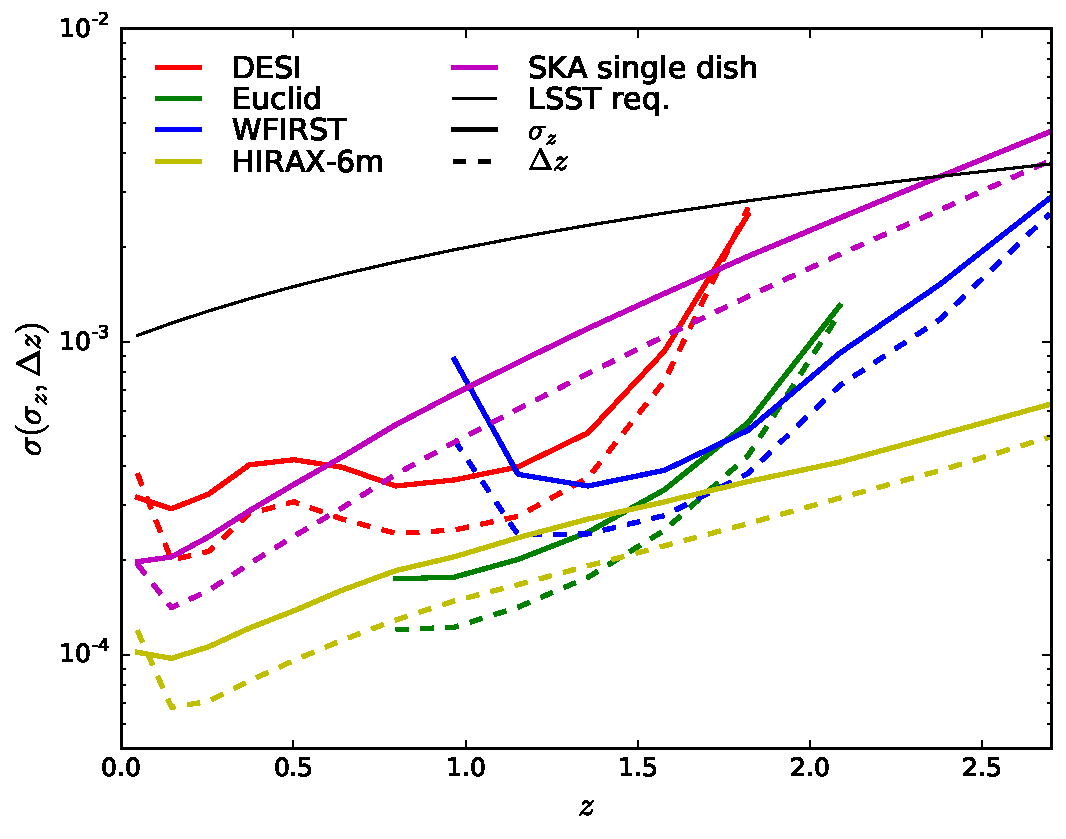
\includegraphics[width=0.49\textwidth]{photoz_calib_compare}
      \caption{\TODO{}}
      \label{fig:fisher}
    \end{figure}

\section{Discussion}\label{ssec:discuss}
  \TODO{\lipsum[12]}

\section*{Acknowledgments}
  We thank Odin the almighty for useful comments and discussions.
 
\bibliography{paper}

\appendix
\begin{widetext}
  \section{Individual clustering redshifts}\label{app:ind_phz}
    \TODO{
      Possibly describe formalism to sharpen redshifts for individual redshifts.
    }
    
  \section{Angular power spectra}\label{app:cls}
    \TODO{
      Describe models used for the angular power spectra
    }
\end{widetext}

\end{document}
